\section{The validation program}\label{sec:validation}

This section designs the studies that would turn gap candidates into validated predictions of
where the Human Knowledge Residual lies (\cref{sec:residual}). \evfut{} Nothing in it has run. It
follows the rules registered in \repo{REORIENTATION.md} (§14, §18, §22) and marks anything new as
\enquote{proposed}. \evobs{} The starting point is a pipeline with one bottleneck. The absence
check (closure) is not yet informative: the judge's verdict does not depend on which evidence it
is shown. All three maps also share one configuration tuned on the same ledgers
(\cref{sec:n3,sec:not-demonstrated}).

The program asks for no money before its cheapest decisive test has run, and each tranche of money
is released only by a gate that reads CONTINUE. It has three phases (\cref{fig:validation}).
Phase~0 tests the absence check before any grant. Phase~1, a lean methods grant, screens the gap
map against several published expert golds. Phase~2 decides H2 with a blind prospective study
sized for the decision.

The studies test the hypotheses of \cref{sec:question} one link at a time; a failed link stops or
reroutes everything above it. The links are trustworthy inputs (L0, V0), an informative absence
check (L1, V1) and retrospective prediction on published gold (L2, V2). Then come a measurable
residual (L3, V4), prospective prediction (L4, V5, which decides H2) and practical value (L5,
V6--V8; V6 tests H3).
\evint{} L1 comes first: with an uninformative closure step, a gold test measures \enquote{a lens
fired} plus density. The developer-departure study (V3) is off this chain: it tests a separate
organizational hypothesis, H-OSS (\cref{subsec:hoss}), and can neither stop nor license H2.

\subsection{Phases, gates and the money they release}

\begin{evfutbox}
  \textbf{Gate rules, proposed for pre-registration.}\\[2pt]
  \textbf{MS1, closure verdict (end of Phase~0).} CONTINUE if human--human $\kappa \geq 0.70$ on
  the gating split, corpus-level retrieval recall meets its pre-registered floor, and at least one
  judge beats the fair control by the pre-registered margin. Otherwise STOP the automated absence
  check.\\[2pt]
  \textbf{MS3, screening gate for Phase~2 money (end of Phase~1).} CONTINUE only if the pooled
  retrospective $\Delta$AUROC has a point estimate $\geq \delta$, \emph{and} its lower 90\% bound
  is $> -\delta/2$, \emph{and} the map adds value over density and area size. Otherwise STOP H2
  funding. MS3 is not a verdict on H2, and it has no inconclusive route: it releases Phase~2 or it
  does not.\\[2pt]
  \textbf{MS5, H2 verdict (Phase~2).} STOP if the upper 90\% bound of the prospective
  $\Delta$AUROC is below $\delta$. CONTINUE if the lower 90\% bound is above 0 and the point
  estimate is at least $\delta$. Any other reading is inconclusive, is reported as not supporting
  H2, and ends H2 funding.
\end{evfutbox}

\paragraph{Phase~0: the closure study, before any grant.} \evfut{} This is the recommended next
action. The owner runs V1 within the NOW program's one permitted human input: a non-owner blind
coder who labels and does not participate. It needs no participants, no gold and no grant: coder
hours and local compute, of the order of EUR~$10^3$. \evint{} Its numbers (human--human $\kappa$,
retrieval recall, and each judge's own-minus-control gap) should be on page~1 of any grant
proposal; this report is the design for them. On STOP, the program takes one of two pivots:
reconstruction with provenance as an audit tool, with no claim about hidden knowledge, or the
interview-only pivot (\cref{sec:roadmap}).

\paragraph{Phase~1: a lean methods grant, released only on MS1 CONTINUE.} About EUR~0.3--0.5\,M
over 12--15 months (\cref{sec:resources}). It builds the area score and freezes the
configuration (MS2). It then validates the adopted judge on the text type of the later studies,
runs V2 pooled over several published CTA golds with V4 on the same data, and ends at MS3. On STOP, H2 funding ends; the
interview-only pivot is costed separately and must stand on its own merits. If H2 fails here, the
money spent on it is Phase~0 and Phase~1 only.

\paragraph{Phase~2: the full program, released only on MS3 CONTINUE.} V5 decides H2 at MS5 and is
budgeted for the power its rule needs. V6 (H3), V7 and the novice study V8c start only on MS5
CONTINUE, each under its own gate. H-OSS (V3) runs on the organizational track once its
components exist.

\paragraph{Who reads the gates.} An independent statistician, or an advisory board with one, reads
MS1, MS3 and MS5 against the pre-registration, with authority over them; any owner exception needs
this reader's sign-off. \evobs{} The N2-to-N3 step was an owner exception without such a reader
(\cref{sec:evolution}), and none is named yet (\cref{sec:team}).

\subsection{Rules common to every study}

\paragraph{Pre-registration and a two-step freeze.} \evfut{} Every threshold, the primary gold,
model and baseline, the area partition and the gap-map configuration are hash-committed before the
data they judge exist \parencite{nosek2018preregistration}. The order is fixed. First, the judge is
chosen at MS1. Then MS2 (about month~4 of Phase~1) hash-commits the V0, V2 and V4
pre-registrations, the lexicons, the thresholds, the adopted judge, the area score and the list of
eligible golds. Only then is gold acquired, and only then are held-out domains reconstructed. A
change after gold is seen makes the result exploratory. H-OSS has its own freeze (MS2b), after its
Git adapter exists.

\paragraph{Area score.} \evobs{} The gap map emits claim-level candidates, cut by a display cap
that drops most PLC candidates, and no area score (\cref{sec:n3}). \evfut{} Every decisive test
ranks \emph{areas}, so Phase~1 builds an area score before MS2. It is a fixed aggregation (for
example the maximum, or a noisy-OR) of per-candidate scores over the \emph{uncapped} lens records in
each area of the registered partition, with a tie rule. It is chosen on pilot data only. Proposed: a map with
more than half its areas tied at zero is uninformative for that gold.

\paragraph{Density and area size.} \evint{} Candidacy and rank are built from source counts, and on
PLC the ranking tracks source density ($\rho = 0.91$, \cref{sec:n3}). A plain $\Delta$AUROC over
density is then close to testing a variable against itself, and a null would be expected by design.
\evfut{} So, before MS2, the area score's partial rank correlation with density and area size is
reported on the pilot ledgers, and the incremental analysis is pre-registered. Primary: the area
score's AUROC \emph{within} density tertiles, pooled over tertiles and golds (the conditional
AUROC). Secondary: the area score's coefficient in a logistic model that already contains density
and area size, with gold as a random intercept.

\paragraph{Domains, dated corpora and memorization.} PLC and GDPR tuned the lexicons, so they serve
only for debugging, the V1 closure set and an unanalyzed V5 pilot. Decisive studies use held-out
domains on a corpus dated before the criterion (\cref{sec:domains}). \evfut{} A dated corpus admits
only sources with a verified date. These are archive captures (Wayback Machine CDX records or
Common Crawl snapshots) taken before the cutoff and used as captured, and publications whose
OpenAlex publication date precedes it. A per-gold blocklist removes the gold paper and its known
citing works. Older procedural text is often paywalled, so before MS2 a metadata-level pilot counts
the dated sources each candidate gold's queries reach; below a pre-registered floor, the gold is not
eligible. \evint{} Memorization cannot be removed: every model postdates the old golds, including
the planner that picks queries. The area partition therefore comes from a dated pre-gold source
by a written procedure, not from a model. Each gold item gets a guided-completion memorization probe
on every model in the chain, and probe-positive items leave the primary analysis
\parencite{golchin2023time,sainz2023nlp}. A plain-LLM ranking without retrieval is a baseline, so
priors alone are scored.

\paragraph{Judges and matchers.} No LLM judge is a criterion. A judge or matcher is adopted only
from a family other than the generator's, with $\kappa \geq 0.70$ against blind human coders and
not below the lower bound of human--human $\kappa$ (the adoption rule). \evfut{} Proposed: before
any gold is unsealed, a stratified sample of closure units from each dated V2 reconstruction, and
later from each V5 domain, is double-coded. Where the adopted judge fails the rule on that text
type, closure there is human-coded, a pre-registered fallback rather than a configuration change.

\paragraph{Statistics.} The headline metric is area-level AUROC, compared by DeLong's method
\parencite{delong1988comparing}, Obuchowski's clustered extension
\parencite{obuchowski1997nonparametric} or a cluster bootstrap. \evfut{} Proposed: the strongest of
the pre-specified baselines is chosen \emph{inside each bootstrap resample}
($\min_k \Delta\mathrm{AUROC}_k$), so the choice is part of the sampling distribution. The MS5 rule
has the logic of two one-sided tests
\parencite{schuirmann1987comparison,lakens2017equivalence,lakens2018equivalence}. Labels use
weighted $\kappa$ or Krippendorff's $\alpha$ \parencite{hayes2007answering,krippendorff2004reliability},
with prevalence beside $\kappa$ \parencite{feinstein1990high} and Wilson intervals
\parencite{wilson1927probable}.

\paragraph{Choosing $\delta$, and planning arithmetic.} \evfut{} Proposed: $\delta = 0.05$ AUROC
(still open in the registered threshold table). A smaller gain over density is unlikely to justify
the reconstruction, while $\delta = 0.10$ would let a stop rule kill a real but modest gain.
Planning uses Hanley--McNeil errors \parencite{hanley1982meaning}, balanced classes, AUROC 0.70
against 0.62 and an error correlation of 0.5; \evint{} these values have no empirical basis. The
90\% half-width of $\Delta$AUROC is then about $\pm 0.14$ with 20 areas per class, $\pm 0.10$ with
40, $\pm 0.08$ with 60, $\pm 0.06$ with 100 and $\pm 0.05$ with about 150. It depends mainly on the
number of areas: a smaller gap (0.66 or 0.62 against 0.62) moves it by under 0.01, and a
correlation of 0.3 widens it by about a fifth. One CTA gold, such as Sullivan's 46-item list
\parencite{sullivan2014use}, gives perhaps 15--25 areas.

\subsection{The studies}

\Cref{fig:validation} shows the phases and gates; \cref{tab:validation} summarizes each study.

\begin{figure}[tbp]
  \centering
  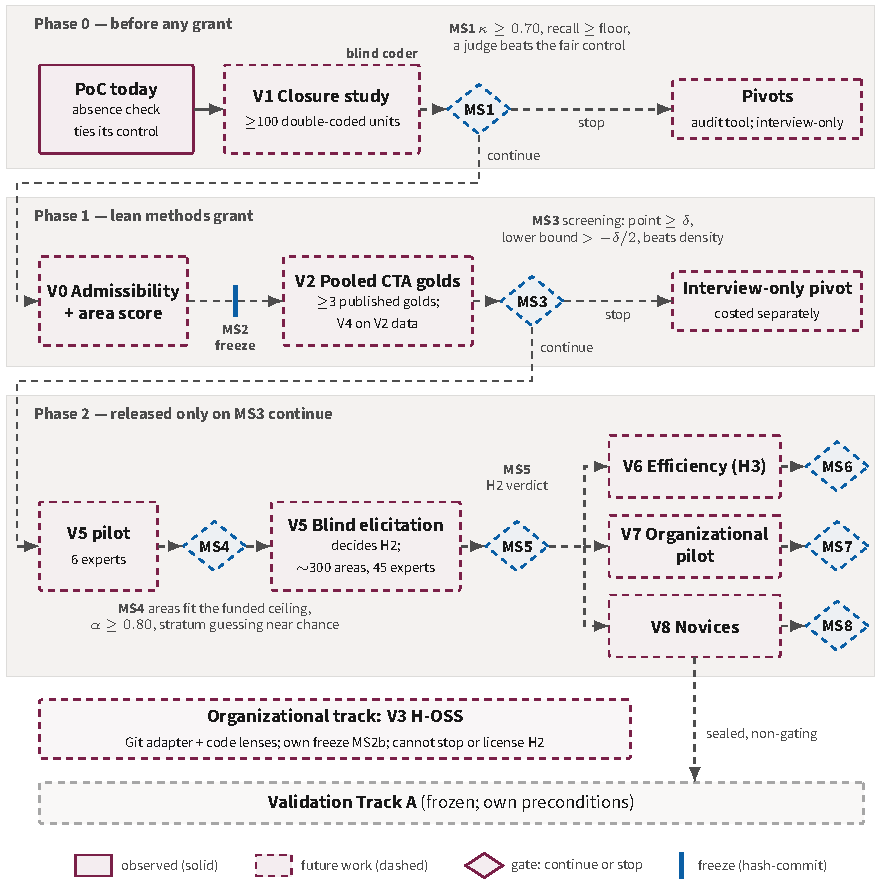
\includegraphics{figures/pdf/fig13_validation.pdf}
  \caption[The validation program]{Which studies, in which order, turn gap candidates into
    validated predictions, and which gate releases which money? Phase~0 (V1, the closure study,
    before any grant) ends at MS1. On CONTINUE, Phase~1 (V0 and the MS2 freeze, V2 pooled over
    several published CTA golds, V4) ends at the MS3 screening gate, which either releases
    Phase~2 or stops H2 funding. In Phase~2, V5 decides H2 at MS5 (after its pilot gate MS4);
    only on CONTINUE do V6 (H3), V7 and V8 follow. V3 sits on the organizational track: it tests
    the separate hypothesis H-OSS and can neither stop nor license H2. A STOP at MS1 leads to
    one of two pivots (an audit tool, or interview-only); a STOP at MS3 leads to the separately
    costed interview-only pivot. Validation Track~A runs on a separate rail on its own
    preconditions and connects only through sealed, secondary, non-gating predictions. All
    elements except the PoC are future work.}
  \label{fig:validation}
\end{figure}

\subsubsection{Phase~0 --- V1 (L1): the closure study}

\emph{Labels and units.} Coders and judges assign \emph{closed}, \emph{partial} or \emph{open},
the three states triage uses. A unit is (lens, seed span, missing element, evidence pool), in the
two arms of the PoC's fair control: own evidence, and evidence swapped from the nearest other
candidate of the same lens. The sample is all 107 admissible PoC firings (PLC 56,
GDPR~v1 51)\footnote{\repo{research/n3/plc/gapmap.json} and the GDPR maps, key
\code{checks.judge_lexical_confusion}.} in both arms: 214 units, and at least 100 double-coded
units if some prove uncodable. About 100 units from one new non-gold domain are added, so that no
judge is scored only in-sample. GDPR~v2's 48 firings (not N3-admissible) serve only for codebook training.
\emph{Coders.} The judgment is textual, so coders need codebook training, not domain expertise. The
non-owner coder and the owner (under origin blinding) code every unit, blind to arm, judge answer,
rank and run. \evint{} The gating $\kappa$ therefore pairs one non-owner coder with the owner;
Phase~1 adds a second non-owner coder.
\emph{Retrieval recall.} \evfut{} The residual requires absence from the whole corpus, not only
from the retrieved pool. So, for a random subset of about 50 firings, the non-owner
coder searches the ledger's full fetched snapshots for the missing element. Retrieval recall is the
share of elements found there that the pool also holds; proposed floor 0.80.
\emph{Judges and measures.} The panel holds the local 7B model, a stronger open-weight model, and
frontier models from families other than the generator's and verifier's (proposed decision 0008).
Primary measure: agreement on the three states (weighted $\kappa$, or ordinal
Krippendorff's $\alpha$), with closed versus not closed, the triage split, as the gating split.
Secondary: the prevalence of \enquote{not stated}, and each judge's own-minus-control difference
against the humans'.
\emph{Sample size.} With classes near balance on the gating split, $\kappa \approx 0.70$ (observed
agreement 0.85, chance 0.50) has a 95\% half-width of about $\pm 0.10$ at 214 units and $\pm 0.14$
at 100. The open state is rare (the judge called 15 of 155 firings open), so its $\kappa$ is wide
at this size (about $\pm 0.17$ at 200 units); it is reported, not gated. Units share seeds, so
$\kappa$ intervals are clustered by seed.
\emph{Gate (MS1).} As in the box. Proposed margin: a judge beats the fair control if its
own-minus-control difference in the not-closed rate has a 95\% lower bound above 0 and lies within
$\pm 0.10$ of the humans' difference. The adopted judge must also meet the adoption rule on the
gating split, on the new domain alone as well as pooled.

\subsubsection{Phase~1 --- V0 (L0): readiness and the deferred N2 validation}

Prepare the MS2 freeze. Implement admissibility as code: every located extraction has a verdict,
the cross-family verifier and the decoys ran (their current stages never ran live;
\cref{sec:architecture}), and completeness comes from the failed-call record. Build the dated-corpus
mode and the area score. N2's registered verdict is INCONCLUSIVE (\cref{sec:n2}); its deferred
protocols (E-LIVE v3, second runs of E-PLANT and E-ABST) run as registered, after a pilot that
prints each gate's best reachable outcome. E-PLANT's validity floor is re-derived from that pilot,
as a registered amendment, because it came from a setting where the planted document was the only
retrieved context. \emph{Gate:} MS2; no hash, no gold. The deferred N2 validation gates V7 and any
provenance claim, not V2.

\subsubsection{Phase~1 --- V2 (L2): pooled replay against published CTA golds}

\emph{Golds and the selection rule.} \evfut{} A gold is eligible if it is an itemized list of
steps, decisions or cues, built by CTA from more than one expert. Its domain must also yield a dated
corpus above the floor and must not be PLC, GDPR or Track~A's physics content, and the gold must be
obtainable for coding. Eligibility is checked by metadata and author contact only,
and the list is fixed at MS2. Named candidates follow, in order. Sullivan's
cricothyrotomy task list is the only one confirmed as itemized \parencite{sullivan2014use}. Then
come the neonatal intensive-care (NICU) cue study \parencite{crandall1993critical}, the troubleshooting study
\parencite{chao1994percentage} and the PARI guide's worked analyses \parencite{hall1995procedural}.
Further CTA-based studies reported in reviews \parencite{clark2008cognitive,tofelgrehl2013cognitive}
have unchecked availability.
Proposed: at least three golds, four to six if eligible. Fewer is reported at MS2; the MS3 rule
does not change, so fewer areas only make CONTINUE harder.
\emph{Design.} For each gold, build the area partition from a dated pre-gold source and
reconstruct from the dated corpus, the gold domain's first and only reconstruction. Run the frozen
gap map and double-code the closure sample; only then acquire the gold, sealed. \evint{} The gold stands in for
$H$, and the reconstruction $R$ is not the evidence base $E$ (\cref{sec:residual}). So each gold
item that $R$ lacks is checked against the dated corpus under the V1 codebook. An area is
\emph{residual-present} only if it holds an important gold item absent from the corpus; items the
corpus states but $R$ missed are scored separately as reconstruction misses.
\emph{Baselines.} The registered baselines, among them random, area size, retrieval-support
density, corpus frequency, a type prior from the other golds (leave-one-gold-out), and a plain-LLM
ranking on a model from another family. Coders see no score, origin or model family; all
item-to-area assignments and at least 20\% of reconstruction--gold pairs are double-coded.
\emph{Analysis.} Primary: the pooled $\Delta$AUROC for residual-present areas against the strongest
baseline, by a random-effects model over golds or a cluster bootstrap with gold as the top-level
cluster. Incremental: the conditional AUROC within density tertiles; the map \enquote{adds value}
at MS3 if its point estimate is at least $0.5 + \delta$.
\emph{Sample size and what MS3 can read.} Three to six golds of 15--25 areas give about 45--150
areas. At four golds and 80 areas split evenly, the half-width is about $\pm 0.10$ before
between-gold heterogeneity. CONTINUE then needs a point estimate of at least 0.075, because the
lower bound must clear $-0.025$. Under the planning assumptions, a map with no true gain passes
with probability about 0.11. A true gain of $\delta$ passes with about 0.34, and one of 0.10 with
about 0.66 (0.13, 0.45 and 0.81 at 60 areas per class). \evint{} MS3 is a screen. It accepts
about a one-in-nine chance of releasing Phase~2 for a map with no gain, which V5 then stops, in
exchange for keeping most large gains. It cannot show that a small gain is absent; that is V5's
job.

\subsubsection{Phase~1 --- V4 (L3): the residual known-truth check}

First a labeled synthetic simulation with planted dependence between occasions (a known-truth use
of synthetic data, not a criterion). Then, on V2 data, capture--recapture estimators that allow
unequal catchability over text occasions are compared with the gold-as-occasion count against a
pre-set tolerance, with Chao1 as a lower bound \parencite{chao1987estimating,briand2000comprehensive}. \evint{} Literature is written by experts, so
occasions are positively dependent and the estimate is biased low; only the known-truth check can
validate it. Out of tolerance, the estimated residual is dropped as an objective and V5 reports
observed counts only. V4 informs MS3's report but does not gate it.

\subsubsection{Phase~2 --- V5 (L4): blind prospective elicitation, which decides H2}

\emph{Design.} Within-expert and area-level. Freeze and hash-commit the reconstruction, dated
corpus, gap map, area score and area partition. Sample areas into four labeled strata: top of the
area score (G), lowest retrieval density (D), top of a plain-LLM ranking (L) and uniform random
(R), plus a pre-registered fraction of confident-but-unverified areas
\parencite{lakkaraju2017identifying}. Sampling spans the whole score range, so $\Delta$AUROC is
estimable with known inverse-probability weights. Each area gets a short probe of about 8 minutes: the same neutral CDM-style question for every area
\parencite{klein1989critical} (\enquote{Walk me through the last time you handled this. What did
you notice? What did you check? What would a newcomer miss?}), never the gap map's own question,
and at most one follow-up restating the expert's words. Each expert covers about 20 areas in two
sessions, balanced across strata, in random order.
\emph{Domains and people.} A PLC pilot, not analyzed for effect; the main study in two held-out
domains with at least 150 areas each at the registered grain (\cref{sec:domains}). Practitioners
with several years of practice, outside any Track~A pool, three per area, the best cost--benefit
point in \textcite{chao1994percentage}. One interviewer per domain, two blind coders, one
validator.
\emph{Outcome.} Expert turns are segmented into items (cue, decision rule, check, rationale,
expectancy). An item counts if it is absent from the frozen reconstruction \emph{and} the dated
corpus under the V1 codebook, and a second expert, a trace or an artifact outside the corpus
corroborates it. Other experts rate importance a week later, blind to stratum. An area is
\emph{residual-present} if it holds at least one validated, important new item.
\emph{Blinding and disclosure.} Experts are told that the study maps where practice relies on
unwritten knowledge, not that a model chose areas. This partial disclosure is stated in the ethics
application; every expert is debriefed afterward and may withdraw their data. The interviewer sees
only area names in random order, coders see pseudonymized turns, and a guess-the-stratum check on
20\% of areas reports leakage.
\emph{Analysis.} Primary: prospective $\Delta$AUROC against the strongest baseline, clustered by
expert and area \parencite{obuchowski1997nonparametric}, with the conditional AUROC within density
tertiles. Secondary: the rate ratio of validated important items, G against the strongest of D, L
and R (mixed-effects negative binomial, \cite{bates2015fitting}), and expert minutes per item.
Segmentation targets $\alpha \geq 0.80$; \enquote{new versus in text} and \enquote{same item} need
$\kappa \geq 0.70$.
\emph{Sample size and expert-hours.} No effect is assumed. MS5 needs a half-width near
$\delta = 0.05$: about 150 residual-present and 150 other areas, so about 300 areas. Three experts
per area make 900 probes. At 20 areas per expert, that is 45 experts (about 22 per domain) plus 6 in
the pilot. Each expert gives about 3 hours in sessions and 1 hour rating other experts' items: about
150--250 expert-hours in all, and about 70 session hours per interviewer. \evint{} Coding costs
more than the experts. About 120 hours of audio must be segmented and matched against the
reconstruction and the dated corpus by two coders: about 1,200--1,900 coder hours. At the rates in
\cref{sec:resources}, honoraria, recruitment and coding come to roughly EUR~40--160k before staff
time. Two things can raise this. If residual-present areas are rarer than half, more areas are
needed (about 500 at a prevalence of 0.3), and clustering by expert adds a design effect.
\emph{Gates.} The pilot (6 experts $\times$ 20 areas: 40 areas, three experts each) estimates
prevalence, design effect, coding time and leakage. \textbf{MS4} releases the main study only if the
projected number of areas fits a funded ceiling of 450 (1.5 times the plan), segmentation reaches
$\alpha \geq 0.80$, and stratum guessing stays near chance. Otherwise V5 stops before the main
study, and H2 is reported as untested prospectively; an underpowered main study is never run.
\textbf{MS5} then reads the rule in the box. At a half-width of $\delta$, every reading is decisive
except a point estimate between 0 and $\delta$.

\begin{table}[tbp]
  \centering\scriptsize
  \caption{The validation studies at a glance. All rows are future work; every rule is
    pre-registered before the data it judges. \enquote{At planned $n$} gives the best reachable
    outcome under the planning arithmetic.}
  \label{tab:validation}
  \begin{tabularx}{\linewidth}{@{}>{\raggedright\arraybackslash}p{0.12\linewidth}
      >{\raggedright\arraybackslash}p{0.10\linewidth}>{\raggedright\arraybackslash}p{0.11\linewidth}
      >{\raggedright\arraybackslash}X>{\raggedright\arraybackslash}p{0.17\linewidth}
      >{\raggedright\arraybackslash}p{0.16\linewidth}@{}}
    \toprule
    Study (link) & Phase / gate & Humans & CONTINUE if & Otherwise & At planned $n$ \\
    \midrule
    V1 Closure (L1) & 0 / MS1 & Owner + 1 non-owner coder & Human $\kappa \geq 0.70$; recall
      $\geq$ floor; a judge beats the fair control by the margin & STOP automated absence check;
      pivots & $\kappa$ $\pm 0.10$ at 214 units \\
    V0 Readiness (L0) & 1 / MS2 & 1 coder (E-ABST) & Runs admissible; MS2 hash; N2 gates as
      registered & No hash: no gold; N2 Stop: no V7 & -- \\
    V2 Pooled CTA golds (L2) & 1 / MS3 (screen) & 2 coders & Pooled $\Delta$AUROC point $\geq
      \delta$, lower 90\% $> -\delta/2$; conditional AUROC $\geq 0.5 + \delta$ & STOP H2 funding;
      separate pivot & $\pm 0.10$ at 40 per class: point $\geq 0.075$ needed \\
    V4 Residual check (L3) & 1 & None & Estimate within tolerance of gold-as-occasion & Drop the
      estimated residual & -- \\
    V5 Prospective (L4; H2) & 2 / MS4, MS5 & 6 pilot + about 45 experts, 3 per area & Lower
      90\% $> 0$, point $\geq \delta$ & Upper 90\% $< \delta$: STOP H2; else not supporting H2 &
      $\pm 0.05$ at 150 per class: decisive unless $0 \leq$ point $< \delta$ \\
    V6 Efficiency (L5a; H3) & 2 / MS6 & 20--30 per domain (illustr.) & Lower 90\% $> 1$, point
      $\geq 1.25$ & Any other reading counts against H3 & Sized from V5 data \\
    V7 Organizational (L5b) & 2 / MS7 & 1 partner, 6--12 staff & G beats D and R in both parts &
      Legal block; not measurable & Descriptive only \\
    V8a Learner data (L5c) & 2 & None & Error excess over difficulty baselines & Null: residual
      $\neq$ learner difficulty & -- \\
    V8b--d Track~A; novices; instruction & Own; 2 / MS8; later & Track~A's own; 30--60 novices &
      K0--K2 unchanged, E-SEAL secondary; novice error excess & Registered rules; no excess & -- \\
    \midrule
    V3 H-OSS (org.\ track) & Org.\ track / MS2b, own gate & 2 coders & Clustered $\Delta$AUROC, MS5
      rule, on H-OSS only & H-OSS stopped; too few departures: descriptive & Set by the
      5-departure pilot \\
    \bottomrule
  \end{tabularx}
\end{table}

\subsubsection{Phase~2 --- V6 (L5a, H3): targeted elicitation efficiency}

Runs only on MS5 CONTINUE, never on an expert's V5 areas. \emph{Selectors, kept distinct.} Two
selectors run as separate arms: the PoC's breadth ranking, as built and frozen, and selection by
expected information gain (EIG) over the gap map \parencite{lindley1956measure,rainforth2024modern},
which is not built. Information-gain questioning has helped in games and preference elicitation
\parencite{piriyakulkij2023active,handa2024bayesian,choudhury2025bedllm}, but no study was found in
expert interviews. A replay without participants (E-EIG) fixes the primary selector before any V6
data. \emph{Design.} Within-expert crossover on matched area sets: block~A targeted
questions, block~B a standard unprompted-then-CDM interview, counterbalanced; proposed third arm, a
plain-LLM list. Items whose content first appears in a question are coded \emph{question-seeded}
\parencite{loftus1975leading} and count only if independently corroborated; Track~A's
leading-question guard is reused by copy. \emph{Measure and gate (MS6).} Validated important new
items per expert hour, ratio A/B for the primary selector; illustration 20--30 experts per domain,
sized from V5's data. CONTINUE if the lower 90\% bound exceeds 1 and the point estimate is at least
1.25. STOP if the upper bound is below 1.25. Any other reading counts against H3.
\evint{} The interview-only pivot reuses this design with EIG over the area partition crossed with
knowledge types and a type prior from the golds, without the reconstruction prior. It is a separate,
separately costed proposal, not a test of H3.

\subsubsection{Phase~2 --- V7 (L5b): organizational pilot}

\evfut{} Runs only on MS5 CONTINUE and after the deferred N2 validation, since partner documents
raise the stakes of prompt injection and false support \parencite{greshake2023not}. In one partner,
it asks whether predicted gaps in critical units match what 6--12 staff experts add in blind
interviews, and where departures or onboarding caused trouble (\cref{sec:organizations}). It runs in
artifact-coverage mode only, under a data-protection impact assessment and, where German
co-determination applies, a works agreement. It reuses the V5 design on one or two units and, if
H-OSS has run, its retrospective design. \evint{} One partner cannot validate a predictor: the pilot
tests feasibility, legal viability and measurability, with the hit rate of G against D and R areas
as a descriptive measure. It goes multi-partner only if G beats D and R in both parts (MS7).

\subsubsection{Phase~2 and later --- V8 (L5c): the learner side, and how Track~A fits}

\evfut{} (a)~In public school-mathematics data, do flagged knowledge components carry more errors
than covered ones, beyond the dataset's own model \parencite{cen2006learning}? It needs no
participants and gates nothing; a null is likely, since the map reads expert-voiced text.
(b)~Validation Track~A runs only on its own preconditions, with K0, K1, K2 and Stage~B unchanged.
The program touches it only through sealed, secondary, non-gating predictions (E-SEAL): an
encrypted, hash-committed file, unsealed after K1 adjudication is locked and matched by coders with
no Track~A role. Anyone who has seen reconstructed conservation content stays ineligible for a
Track~A human role. (c)~On MS5 CONTINUE,
30--60 novices test whether confirmed residual areas show more novice errors than matched covered
areas (MS8). (d)~Much later comes instruction from validated items only, with delayed transfer
(\cref{sec:education}), where CTA-derived instruction has precedent
\parencite{feldon2010translating}.

\subsubsection{Organizational track --- V3: the separate hypothesis H-OSS}\label{subsec:hoss}

\emph{Hypothesis (H-OSS).} The gap map, adapted to code and commit evidence, predicts where
knowledge is lost when developers leave, beyond authorship concentration. \evint{} This is a
different construct from the HKR, measured with a different gap map. So H-OSS can neither stop
nor license H2, and its result is reported only as a reading on H-OSS.
\emph{Components (none exists).} (i)~A World~B Git adapter that turns commits, issues, pull
requests, reviews and dated documentation into claim records with exact spans keyed to a commit
hash or URL. (ii)~Areas mapped to code units existing at a time $t$ before
the departure. (iii)~Lens rules for code text; for example, WHY fires on a change whose commit, pull-request
and issue text give no reason, and GUARD on a special-case branch whose comment or commit names no
condition. Code-text lexicons are developed on repositories outside the
departure sample. The judge is validated on commit and issue units from such repositories; if none
passes, H-OSS is registered without closure (lens firing plus coverage only), a narrower claim.
All of this is frozen at MS2b, after the adapter exists.
\emph{Design.} As registered. Freeze each repository at $t$ and compute the adapted map from
artifacts dated no later than $t$. The outcome is blind, double-coded rationale-seeking
issues and defect-fix commits per unit of later activity, as a difference-in-differences with a
staggered-adoption estimator \parencite{callaway2021difference}. Departures come from truck-factor corpora
\parencite{avelino2016novel,avelino2019abandonment}. Baselines: prior trouble, size, churn,
documentation density, truck factor, knowledge at risk from turnover-loss studies
\parencite{rigby2016quantifying,nassif2017revisiting}, and a plain-LLM ranking. Blind outcome
coders reach $\kappa \geq 0.70$ on 200 stratified issues. Developers are pseudonymized data
subjects.
\emph{Sample size and gate.} The effective sample is near the number of departures. A 5-departure
pilot estimates the base rate, the within-repository correlation and coding time, and from them the
departures needed for a clustered 90\% half-width no wider than $\delta$. The main study runs only
if that many departures with enough later activity exist (the registered expectation is tens);
otherwise H-OSS is descriptive. Its own gate uses the MS5 rule.

\subsection{Threats to the validity of the program, and mitigations}

Contamination and in-sample tuning are treated with the PoC's threats (\cref{sec:threats}). Four
threats are specific to measuring the residual.

\paragraph{The gold is incomplete.} $H$ is what a few experts said and did, so true residual items
outside it look like false positives. Hence three experts per area as a floor
\parencite{chao1994percentage}, $R \setminus H$ reported but never as error, saturation checks that
allow for plateaus \parencite{guest2020simple,hennink2022sample}, and no residual declared zero.

\paragraph{The method shapes $H$.} Prompting changes how much experts report (\cref{sec:problem}),
verbal reports can be wrong \parencite{nisbett1977telling}, directed explanation can change what
experts do \parencite{fox2011procedures,ericsson1980verbal}, and leading questions can plant content
\parencite{loftus1975leading}. The measured HKR is always \enquote{the residual as revealed by
method $M$}, a lower bound, and V5's short probes make it a conservative one. Hence neutral probes,
question-seeded coding and corroboration.

\paragraph{The matcher can err or become the gold.} A lenient matcher shrinks the residual, a
strict one inflates it, and an unchecked LLM matcher silently becomes the criterion. Hence the
adoption rule and its re-check on each text type, matchers blind to scores and origin, and
contradicted items recorded as contradictions. Results compare only at a fixed, dated $E$.

\paragraph{People and governance.} A frozen codebook, origin blinding, non-owner gating coders and
random area order guard against drift, owner knowledge and fatigue. With one interviewer per domain,
the claim is \enquote{with this interviewer}.
Ethics approval covering V5's partial disclosure precedes V5; an impact assessment and a works
agreement precede V7. A study stopped by budget or law is reported as stopped, never
reinterpreted.

\evint{} Each STOP teaches something. At MS1, it shows that absence in text cannot yet be judged
reliably, and it leaves a public closure set. At MS3, it leaves a reconstruct-versus-CTA benchmark.
At MS5, it falsifies the claim that text reconstruction locates the human residual, with a bounded
effect size.
